\documentclass{beamer}
\usepackage{amsmath}
\usetheme{Berlin}

\begin{document}

\author{Josh Borrow}
\title{Supernovae and Isotropy}
\date{\today}

\maketitle

\frame{\frametitle{Contents}\tableofcontents}

\section{Fitting $\Lambda$CDM with $k\neq0$}

\frame{\frametitle{Fitting the Friemdann equation}
\begin{equation}
    \frac{H^2}{H_0^2} = (\Omega_b + \Omega_C)a^{-3} + \Omega_ka^{-2} + \Omega_\Lambda~.
\end{equation}
}

\frame{\frametitle{Comoving Distance}
\begin{align*}
	r(z) = \frac{c}{H_0 | \Omega_k |^{1/2}} \mathrm{sinn}\left(|\Omega_k |^{1/2} \int^z_0 \frac{\mathrm{d}z'H_0}{H(z')}\right)~.
\end{align*}
Where sinn is defined as sinh for $\Omega_k > 0$ and sin for $\Omega_k < 0$, for $\Omega_k=0$ this reduces to the integral and $c/H_0$ prefactor (Weinberg 1972).
Computational precision used $1\times10^{-9}$ for checks (even though they reduce to the same thing as $\Omega_k \rightarrow 0$).
}

\frame{\frametitle{Data}
\begin{itemize}
     \item Union 2.1 Compilation
     \item 580 supernovae
     \item redshift 0.015 to 1.414
\end{itemize}
}

\frame{\frametitle{Fitting}
\begin{figure}
    \centering
    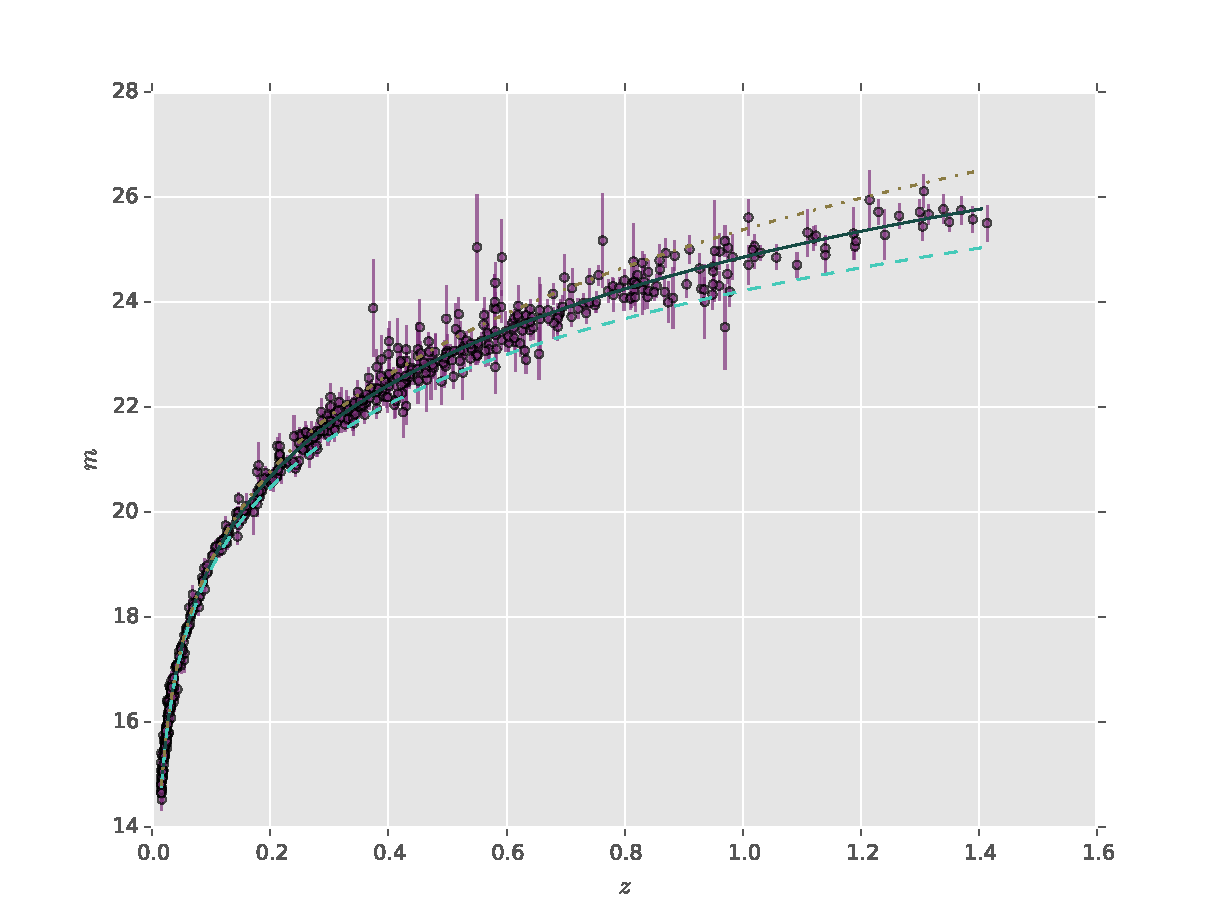
\includegraphics[width=0.7\textwidth]{../figure_1.pdf}
    \caption{Mustard dot-dash (0, 1, 0), light blue dash (1, 0, 0), green solid best fit ~(0.3, 0.7, 0) with these ($\Omega_{b+C}$, $\Omega_\Lambda$, $\Omega_k$)}
\end{figure}
}
 
\frame{\frametitle{Residuals}
\begin{figure}
    \centering
    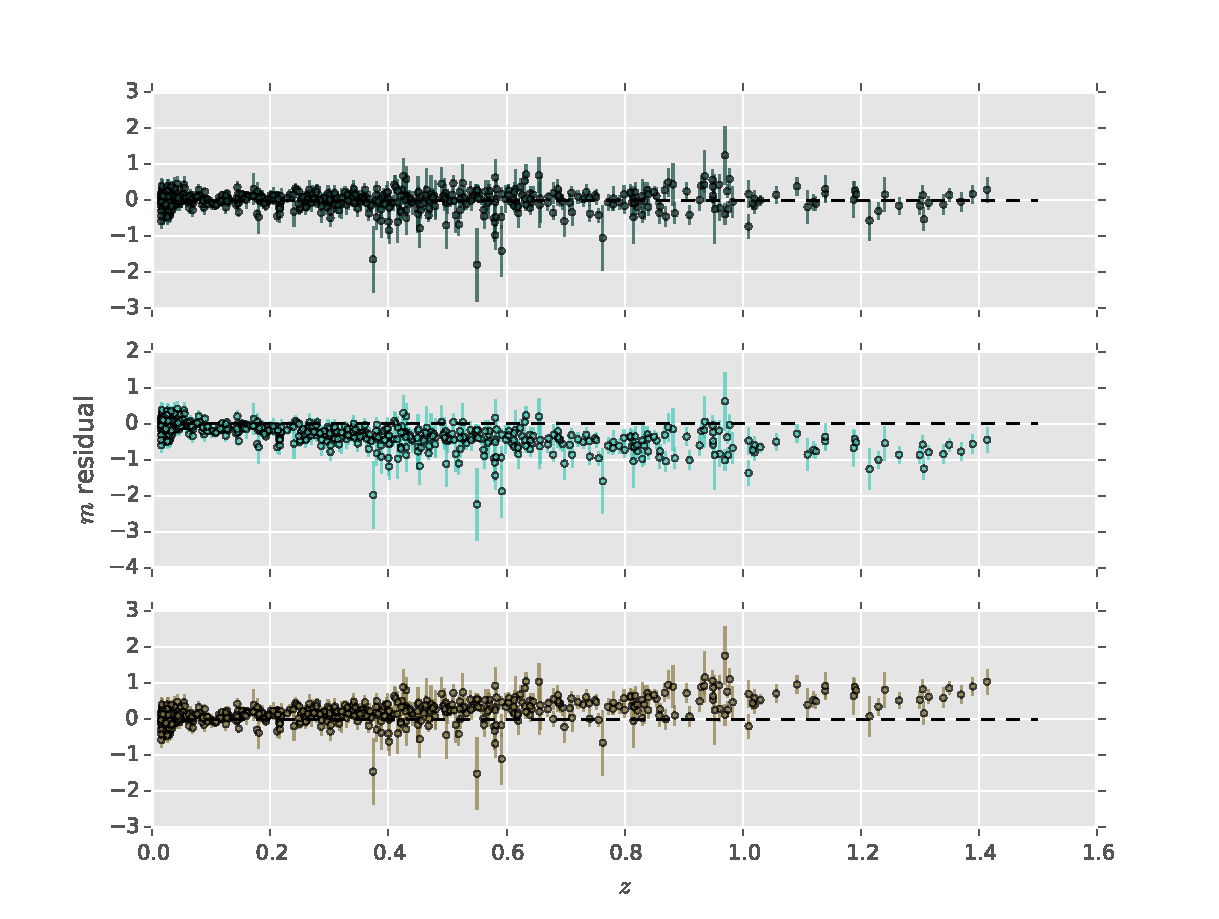
\includegraphics[width=0.7\textwidth]{../figure_2.pdf}
    \caption{Colours the same as previous plot.}
\end{figure}
}

\frame{\frametitle{Results}
\begin{itemize}
    \item $\chi^2_{red} = 0.985$
    \item $\Omega_b + \Omega_C = 0.274(26)$
    \item $\Omega_k = 3\times10^{-6} \pm 0.05$ consistent with 0
    \item $\Omega_\Lambda = 0.726(33)$
\end{itemize}
}

\frame{\frametitle{Difficulties}
\begin{itemize}
    \item Hyper sensitive to initial conditions - many local minima
    \item With this much data computation time is growing (several minutes on laptop) so can spiral easily
    \item The errors on supernovae are too high for this kind of work!
\end{itemize}
}

\frame{\frametitle{What are those?!}
\begin{figure}
    \centering
    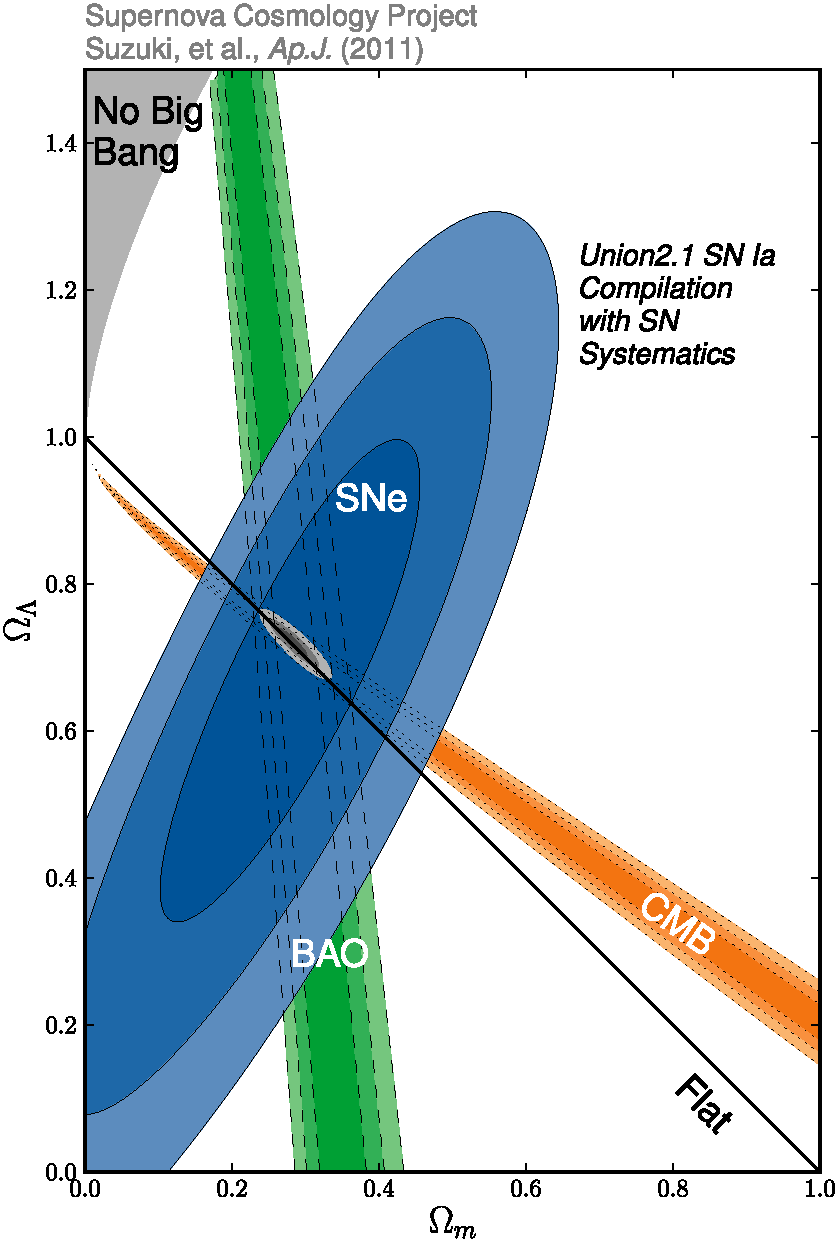
\includegraphics[width=0.4\textwidth]{../figure_3.pdf}
    \caption{From Union 2.1 (2011)}
\end{figure}
}

\section{Isotropy and Future Work}

\frame{\frametitle{Isotropy}
    We can study Isotropy with supernovae!
    
    Write:
    \begin{equation}
	    \mu_{th} = \bar{\mu}_{th} ( 1 + D(\hat{n} \cdot \hat{p}))~,
    \end{equation}
    $\hat{n}$ dipole direction and $\hat{p}$ supernova direction, with $D$ magnitude (Lin et al. 2015).
}

\frame{\frametitle{So what?}
    Look at systematics to find how we need to change them to see anisotropy.
    
    E.g. what if dust absorption is locally more anisotropic than previously thought?
}

\frame{\frametitle{Future Work}
    \begin{itemize}
        \item Look at other datasets (JLA)
        \item Combine data from PLANCK, JLA/Union (SN1a), BAO
        \item Investigate significance of covariance between parameters in model
        \item Anisotropy tests on SN1a data
        \item Anisotropy tests on BAO?
    \end{itemize}
}

\end{document}
